\documentclass[spanish]{article}
\usepackage[T1]{fontenc}
\usepackage[utf8]{inputenc}

\normalsize

\parindent = 0mm 

\usepackage{lmodern}
\usepackage[a4paper]{geometry}
\usepackage[spanish]{babel}
\usepackage{graphicx}
%\usepackage{url}
%\usepackage{booktabs}
%\usepackage{multicol}
%\usepackage{multirow}
%\usepackage[x11names,table]{xcolor}
%\usepackage{float}
%\usepackage{amsmath, latexsym, amsfonts, amssymb} 
%\usepackage{multicol}
\usepackage[shortlabels]{enumitem}
\usepackage{tikz}
\usepackage{floatrow}
%\usepackage[small,bf,labelsep=period]{caption}
%\usepackage[backend=biber]{biblatex}

\bibliography{referencias}

\title{Proyecto de Modelos de Matemática Aplicada. \\Construcción y graficación de grafos causales}

\author{ Dennis Fiallo Muñoz \\ Lauren Guerra Hernández}

%\institute{Facultad de Matemática y Computación de la Universidad de La Habana}

\begin{document}
	
\maketitle


\section*{Presentación del problema}

El usuario necesita construir grafos causales de dos tensores de 360x360xlags, siendo uno binario indicando si hubo conexión o no, y otro de pesos indicando la fuerza de las conexiones. Estos se construyen de la siguiente manera:

\begin{itemize}
\item	Conexiones contemporáneas: Se representan con una línea recta. Se toma el lag 0(único lag simétrico) y donde aparezca 1 significa que hay conexión entre los nodos (i, j), mientras que el color de la conexión que se traza viene dado por el valor de la matriz de peso en la posición (i, j).
\item	Lagged connections o causalidad: Se representan con flechas. Para el resto de lags se busca igualmente si hay un 1 en el tensor binario de 
lag$\neq $0 y se construye una flecha del nodo i al j con 
la intensidad dada por el promedio de los valores de la matriz de pesos en los lags donde hubo conexión, además de especificar los lags con conexión.
\end{itemize}

\begin{figure}[h]
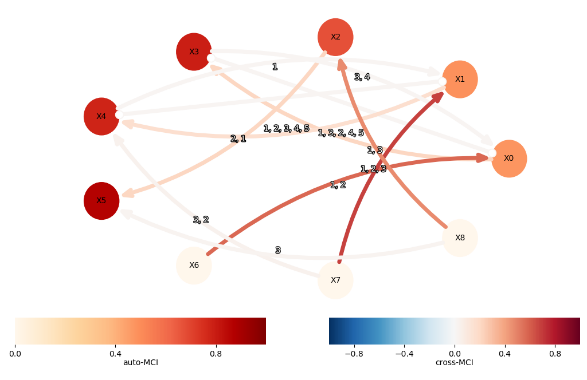
\includegraphics[scale=0.95]{example1.png}
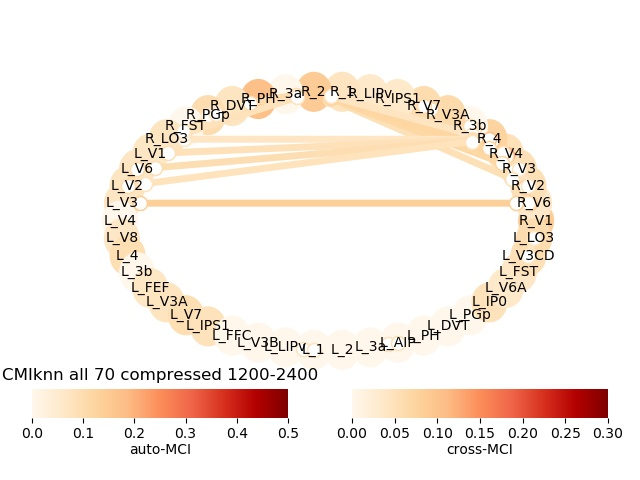
\includegraphics[scale=0.45]{example.png}
\caption{Ejemplo de graficación de un grafo causal admisible}
\end{figure}

\newpage

\subsection*{Problema}

Al pasarle un gráfico de más de 180 series de tiempo(en la práctica se necesitan 360), el programa pone 180 nodos sobre una circunferencia y los restantes los sobrepone a estos en la misma circunferencia, haciendo que no sea posible ver las conexiones.\\


\begin{figure}[h]
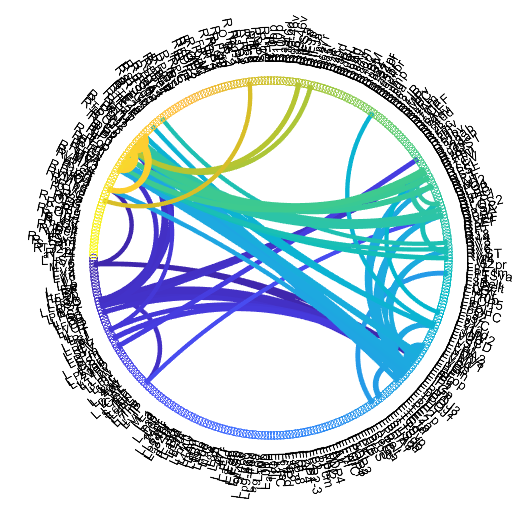
\includegraphics[scale=0.3]{example2.png}%{Ejemplo de graficación en que los nodos se superponen y no se pueden observar los resultados}
\caption{Ejemplo de graficación en que los nodos se superponen y no se pueden observar los resultados}
\end{figure}
 
 
\subsection*{Objetivo}
Hacer un programa al cual se le pasen dos tensores de conectividad y una lista con los nombres de los nodos y construir un grafo como se explicó anteriormente que admita las 360 necesarias y se puedan ver correctamente los nodo, las conexiones y la fuerza de estas.

\section*{Primeras ideas}

Al comienzo de la realización de este proyecto se tenía en mente la implementación de métodos para dibujar grafos que lograran una buena ditribución de nodos y aristas en el espacio bidimensional utilizando los conocimientos adquiridos en asignaturas como Matemática Discreta II, Estructura de Datos y Algoritmos II y Modelos de Optimización, esto dibujando el grafo en su forma maximal planar y luego ir añadiendo las aristas que falten por dibujarse  minimizando la cantidad de aristas que serían dibujadas cortando a las que ya estuvieran colocadas. \\

Esto tuvo grandes inconvenientes porque los grafo causales están muy lejos de ser planares, tienen muchas aristas y a la hora de acomodar los nodos y dibujar las aristas que no formaban parte del grafo maximal planar tomado como base no se podían garantizar distrubuciones de nodos y aristas que garantizaran la correcta observación del grafo.\\

Buscando en el estado del arte no existía nada como esto, ninguna distribución que se hiciera a un grafo resultaba buena en todos los casos, para todo tipo de grafos, probamos con la librería networkx las diferentes distribuciones que esta tiene implementadas y ninguna de ellas cumplía nuestro objetivo, por lo que llegamos a la conclusión que crear un algoritmo que graficara cualquier grafo de la mejor manera poible para él es un ejercicio muy complicado por lo cual no se encontraba a nuestro alcance.\\

Por esto nos propusimos utilizar las mejores implementaciones de dibujo de grafos que estuvieran disponibles en librerías de python para poder resolver el problema del usuario y lograr ssatisfacción\\


\section*{Solución}


\end{document}